\documentclass[]{report}

\renewcommand{\thesection}{\arabic{section}}
% \usepackage[ngerman]{babel}
\usepackage{graphicx}
\usepackage{tabularx}
\usepackage{float}
\usepackage{listings}
\usepackage{url}

\setcounter{figure}{0}

\lstdefinestyle{json}{
  basicstyle=\small\ttfamily,
  showstringspaces=false,
  breaklines=true,
  frame=lines
}

\title{App development for Charité Emergency Department}
\author{Jannes Volkens}
\date{\today}

\begin{document}
\maketitle

\section{Introduction}
This project report is about an app for the Charité Emergency Department, which was created in a collaboration with the Charité. The project was scheduled for the whole semester WS 22/23. This report goes into detail about the background, as well as the implementation, which is followed by a conclusion and an evaluation of the duration of the project.

\section{Background \& Healthcare in ED}
When patients visit the emergency department, they usually receive only a physical doctor's letter and verbal instructions to follow, when they're being discharged. However, this can often lead to problems, as there may be language barriers and instructions can easily be forgotten. In addition, the situation is made more difficult because most instructions are customized for each patient. This can result in confusion and even lead to patients returning to the emergency department to ask for instructions or to see doctors again for examination because they are not feeling better.

\section{Our Objectives \& Team organization}
The objective of this project is to develop a backend application that simplifies the discharge and instructions process for both doctors and patients. The application will allow doctors and patients to log in using their respective login credentials to perform various actions or access information. Doctors will have the ability to digitally hand over doctor's letters to patients, which can be downloaded and then forwarded, or shown to their general practitioners. Additionally, doctors will be able to send patients personalized instructions digitally to reduce the possibility of errors due to language barriers or forgetting the instructions. The system will also provide patients with the ability to send feedback to the ED after a specific period, which includes their post-treatment status. Moreover, the system should send reminders to patients to contact specialists or similar after a specific time. By achieving these objectives, the discharge and instructions process will be simplified, and doctors and patients will have an improved digital experience.\\
Throughout the project we have established a relatively strict organized team structure. Weekly meetings with the Charité were held to discuss open questions and our progress. In these meetings, goals were clarified, and feedback was obtained, which helped us to proceed further. In addition, we almost held weekly meetings within the team to distribute task packages and clarify open implementation questions. Moreover, we also had almost weekly meetings as part of the module to discuss our progress with Professor Wolter and obtain feedback for our continued work. In these we had the opportunity to address any concerns and receive guidance. To manage our work effectively, we utilized WhatsApp and Discord as communication platforms and GitHub to manage our code and individual issues and merge requests. These tools enabled us to keep track of our progress and ensure that the project remained organized and well-managed.

\section{Implementation}

\subsection{Technical background}
\textbf{Java Spring Boot}\\
Java Spring Boot is a popular open-source framework for building backend web applications. It is built on top of the Spring framework, which is widely used for enterprise-level applications. Spring Boot makes it easier to create stand-alone, production-grade applications that can be deployed and scaled easily. The framework provides a wide range of features and functionality, including web applications, messaging, and data access.\\
One of the key advantages of Spring Boot is that it requires minimal configuration, allowing developers to focus on writing application code rather than setting up infrastructure. Spring Boot's auto-configuration feature automatically configures various components based on the libraries available in the project's classpath. This means that developers can quickly create a new project and start building features without spending time on configuring boilerplate code.\\
Spring Boot also comes with an embedded web server, which allows developers to quickly run and test their applications without needing to install a separate web server. Additionally, Spring Boot supports a range of other libraries and frameworks, making it an excellent choice for developers who want to build scalable and maintainable web applications \cite{spring-io}.\\\\
\textbf{FHIR}\\
Fast Healthcare Interoperability Resources (FHIR) is a standard for exchanging healthcare information electronically. FHIR was developed by the non-profit organization Health Level Seven International (HL7) and is based on modern web technologies such as RESTful web services, JSON, and XML. FHIR aims to simplify interoperability between healthcare systems and to make it easier for healthcare providers to access and exchange health data.\\
FHIR provides a standardized format for healthcare data, enabling healthcare providers to share patient information with each other, even if they are using different electronic health record (EHR) systems. FHIR resources define the data elements that can be shared, such as patient demographics, clinical observations, and laboratory results. FHIR also defines the standard operations that can be performed on these resources, such as read, search, and update.\\
FHIR has gained popularity due to its flexibility and ease of use. FHIR resources can be easily integrated into existing healthcare systems and can be accessed using modern web technologies. FHIR also allows developers to create custom profiles, enabling them to define additional data elements specific to their use case. Additionally, FHIR has a growing ecosystem of tools and resources that make it easier for developers to implement the standard and to build applications that use FHIR data. Overall, FHIR is a promising standard for improving healthcare interoperability and enabling better access to health data \cite{hl7-fhir}.\\
For the application, we mainly used three different FHIR resources that can reference each other with their FHIR IDs:
\begin{itemize}
    \item \textbf{Patient:} The Patient resource (see Listing \ref{lst:patient_example}) represents an individual person who is receiving or has received healthcare services. This resource contains basic demographic information about the patient, such as their name, gender, birth date, and contact information. It may also include more detailed clinical information, such as their medical history, allergies, and current medications \cite{hl7-fhir}. \begin{lstlisting}[style=json, label=lst:patient_example, caption={Example for a FHIR patient ressource}]
        {
            "resourceType": "Patient",
            "id": "example",
            "name": [
                {
                    "family": "Smith",
                    "given": [
                        "John",
                        "Doe"
                    ]
                }
            ],
            "gender": "male",
            "birthDate": "1985-01-01",
            "address": [
                {
                    "use": "home",
                    "line": [
                        "123 Main St"
                    ],
                    "city": "Anytown",
                    "state": "NY",
                    "postalCode": "12345"
                }
            ],
            "telecom": [
                {
                    "use": "home",
                    "system": "phone",
                    "value": "555-555-5555"
                }
            ],
            "active": true
        }
    \end{lstlisting}
    \item \textbf{Encounter:} The Encounter resource (see Listing \ref{lst:encounter_example}) represents a healthcare interaction between a patient and one or more healthcare providers. This can include in-person visits, phone calls, videoconferences, and other types of interactions. The Encounter resource contains information about the time and location of the encounter, the reason for the encounter, and the healthcare providers involved. It may also include information about any procedures, diagnoses, or medications that were discussed or performed during the encounter \cite{hl7-fhir}. \begin{lstlisting}[style=json, label=lst:encounter_example, caption={Example for a FHIR encounter ressource}]
        {
            "resourceType": "Encounter",
            "status": "finished",
            "subject": {
                "reference": "Patient/7341361"
            },
            "period": {
                "start": "2023-02-06T08:00:00+00:00",
                "end": "2023-02-06T11:30:00+00:00"
            },
            "type": [
                {
                    "coding": [
                        {
                            "system": "http://terminology.hl7.org/CodeSystem/v3-ActCode",
                            "code": "IMP",
                            "display": "inpatient encounter"
                        }
                    ],
                    "text": "Inpatient Encounter"
                }
            ]
        }
    \end{lstlisting}
    \item \textbf{Condition:} The Condition resource (see Listing \ref{lst:condition_example}) represents a clinical condition, problem, diagnosis, or other issue that is affecting a patient's health. This resource contains information about the condition, such as its name, severity, onset date, and any associated symptoms or complications. It may also include information about the underlying cause of the condition, as well as any treatments or interventions that have been prescribed or performed. The Condition resource is typically associated with a specific patient, and may be referenced in the context of an Encounter or other clinical resource \cite{hl7-fhir}.\begin{lstlisting}[style=json, label=lst:condition_example, caption={Example for a FHIR condition ressource}]
        {
            "resourceType": "Condition",
            "code": {
                "coding": [
                    {
                        "system": "http://snomed.info/sct",
                        "code": "16603009",
                        "display": "Broken leg"
                    }
                ]
            },
            "encounter": {
                "reference": "Encounter/7497538"
            },
            "subject": {
                "reference": "Patient/7341361"
            },
            "onsetDateTime": "2020-03-01T10:00:00+01:00",
            "verificationStatus": "confirmed",
            "clinicalStatus": "active"
        }    
    \end{lstlisting}
\end{itemize}
\textbf{Hapi-FHIR}\\
The HAPI FHIR Test Server is an open-source software tool that provides a platform for testing applications that use the Fast Healthcare Interoperability Resources (FHIR) standard. The Server allows developers to test their FHIR applications in a simulated environment that mimics a real-world FHIR server. This allows developers to verify that their applications can interact with a FHIR server in the way they expect before deploying the application to a production environment. It provides a web-based user interface that allows developers to interact with the server and explore the available FHIR resources. It also provides a RESTful API that developers can use to interact with the server programmatically \cite{hapi-fhir}. This server was used to test the code and add various required FHIR resources.\\\\
\textbf{JWT-Token}\\
JSON Web Tokens (JWT) are a type of token-based authentication mechanism that are widely used in modern web applications. A JWT token consists of three parts: a header, a payload, and a signature. The header contains information about the type of token and the cryptographic algorithm used to secure it. The payload contains the user's identity and any additional data that needs to be transmitted, such as authorization or session data. The signature is created using a secret key that is shared between the server and the client, and is used to verify the authenticity of the token. JWT tokens are typically used for authentication and authorization purposes. When a user logs in to a web application, the server generates a JWT token and sends it to the client. The client then includes the token in each subsequent request to the server, and the server uses the token to verify the user's identity and access permissions. Because the token is cryptographically signed, the server can trust that the data contained in the token has not been tampered with. JWT tokens are popular because they are stateless, meaning that the server does not need to store session data or maintain any state between requests. This makes them more scalable and easier to deploy in a distributed environment. Additionally, because the token contains all the necessary information, it can be used across different domains and services, making it a versatile authentication mechanism \cite{jwt-io}.

\subsection{Databases}
\textbf{Encounters}\\
This database stores the individual encounters (hospitalizations) of the patients. This includes a date when the encounter took place, as well as a list of conditions (diagnoses) that were detected at the respective encounter. In addition, the records contain a list of instructions and a file representing the doctor's letter.\\\\
\textbf{Instructions}\\
This database contains information about what each instruction is called and what its content is. They also contain when the respective instruction was created and by whom (which practitioner) it was created.\\\\
\textbf{InstructionsToPatient}\\
This database contains a bit more information regarding the instructions. Practitioners' comments and patients' feedback for the instructions are included here.\\\\
\textbf{PatientData}\\
This database contains the patient-specific information. Here are the instructions, as well as the individual Encounters contained.\\\\
\textbf{UserData}\\
This database contains the user specific data. This can be data from all roles: Admin, Practitioner, Patient. Included is information such as name, phone number, mail address, as well as the role and the encrypted password.

\subsection{User access \& Security}
\begin{itemize}
    \item Vielleicht noch code?
\end{itemize}
During the project, two different implementations were used for security and login mechanisms to enable secure communication between users and the server. Initially, Spring Security Login was used, a server-side mechanism where the user's authentication state is stored on the server, usually in one session. However, this can be a problem as the number of users grows, as server-side session management becomes more complex and can lead to scaling issues. Therefore, JWT was finally used because it avoids the scalability issues associated with server-side session management and allowed us to store authentication information in a token that is sent with each request from any user. This token contains all the necessary information about the user's identity and permissions, so the server does not need to store any session data. What has not changed is that the login is a Role based login. In total, there are three different roles:
\begin{itemize}
    \item Admin
    \item Practitioner
    \item Patient
\end{itemize}

\subsection{Instructions}
The instructions are there to give the patients their instructions depending on the disease. For the instructions assigned to a patient by a practitioner, some fields are set in the related databases e.g. from which the title, the content, who the instruction is from, when it was assigned, when feedback should be given, etc.. This information can then be viewed by the associated patient or admins. When a patient then views their Encounter instructions, timestamps can then be compared to when feedback is to be given to prompt patients to provide feedback. The instruction entries can also subsequently store the feedback given and the patient's rating.

\subsection{Admin}
Administrators are mainly there to manage all other user accounts, whether Practitioner or Patient, which is all handled by the \textit{AdminController}. Practitioner users can be created and Practitioner and Patient users can be deleted. Administrators also receive feedback from patients regarding their health conditions. By default, there is an admin account with a default login in the code, so that the admin can log into the system after a system start.\\
To manage all user accounts an admin sees two lists: one list shows all existing practitioners with their names, mail addresses and phone numbers and the other list shows all existing patients also with names, mail addresses and phone numbers (see Figure \ref{fig:admin_dashboard}). Calling the Admin Dashboard sends a GET request to the AdminController, which responds with two lists containing all Practitioners and Patients. For this reply, all database entries for the user roles Practitioner and Patient are loaded in the controller. When new users are added, they appear at the bottom of the list as a new entry.\\
\begin{figure}[h]
    \centering
    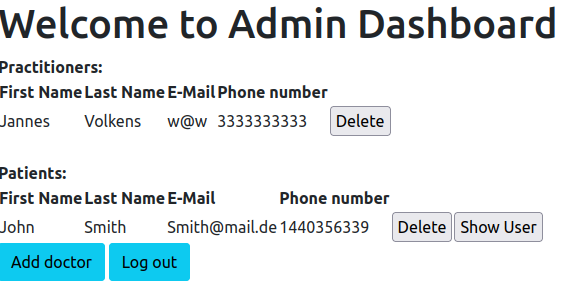
\includegraphics[width=0.6\textwidth]{Admin_Dashboard.png}
    \caption{Admin dashboard with one practitioner and one patient present.}
    \label{fig:admin_dashboard}
\end{figure}
Administrators have the possibility to delete individual users by pressing a button of the respective entry to delete it. Now the AdminController receives the name of the entry and the phone number in a POST request and based on this information the corresponding user is deleted in the database. For the patient entries there is also the possibility to get more information about the respective patient by pressing a button. Here a GET request is sent to the controller containing the associated patient ID, which loads a more detailed patient overview. In this patient overview all encounters of the respective patient can be seen. Information such as the date of the encounter, the diagnoses (conditions), the assigned instructions (title and content), practitioner comment and the patient's feedback (rating and comment) can be seen (see Figure \ref{fig:patient_overview}). There is also the possibility to acknowledge the patient's feedback.\\
\begin{figure}[h]
    \centering
    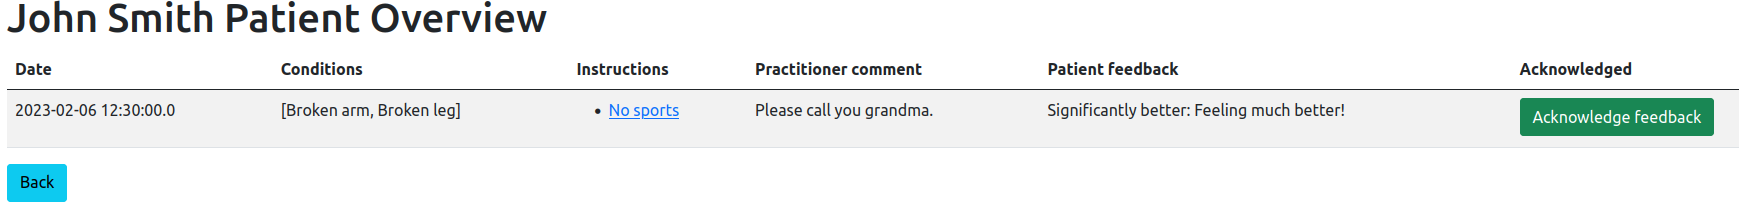
\includegraphics[width=1\textwidth]{Patient_Overview.png}
    \caption{Admin's patient overview.}
    \label{fig:patient_overview}
\end{figure}
If a new Practitioner is to be created, some information about this person must be provided: First and Last name phone number and mail address (see Figure \ref{fig:add_practitioner}). These are then sent to the AdminController via a POST request, whereupon a new user is created with the role of a Practitioner and the specified information. In addition, a password is created for the practitioner, which consists of the first and last name and a 6-digit random number connected by underscores (example: Max\_Mustermann\_123456). If this user already exists, there will be an error output and the user will not be created. After the new Practitioner has been created, the Admin will see as confirmation a small overview for which Practitioner an account has been created and its password.\\
\begin{figure}[h]
    \centering
    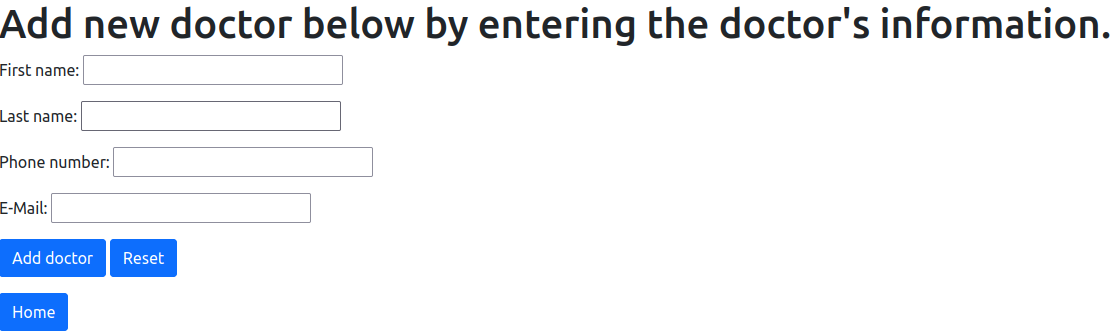
\includegraphics[width=1\textwidth]{Add_Practitioner.png}
    \caption{Interface to add a new practitioner.}
    \label{fig:add_practitioner}
\end{figure}

\subsection{Practitioner}
When patients have finished being treated and can be discharged, the Practitioner-User role comes into play, which the \textit{PractitionerController} controls. They can create new patient users and assign individual instructions to these users. There is also the option of assigning a digital doctor's letter to the patients. The created patient users can then log in to the service and view their assigned instructions and doctor's letters.\\
There are two different types of instructions that can be assigned to patients:\\
\begin{itemize}
    \item Individual instructions where a title and content can be added. The title can be short and concise to make the instruction easily recognizable and the content can contain more information.
    \item Instructions that are fetched from a FHIR server. However, these are exclusively medication instructions, since FHIR does not offer the possibility to store/retrieve other types of instructions. Here a list of all medication instructions is loaded, from which the required ones are selected and can also be edited again.
\end{itemize}
All created and selected instructions appear on the Practitioner Dashboard in a list that contains various information about the instructions, such as an ID for the respective instruction, the title, the content, the author and the time of creation (see Figure \ref{fig:practitioner_dashboard}). The titles of the instructions are links that lead to another view of the respective instruction. The information on the dashboard is obtained here via GET requests to the Practitioner controller. The request returns a list of all the instructions that have already been added and information about the respective Practitioner from the corresponding databases.\\
\begin{figure}[h]
    \centering
    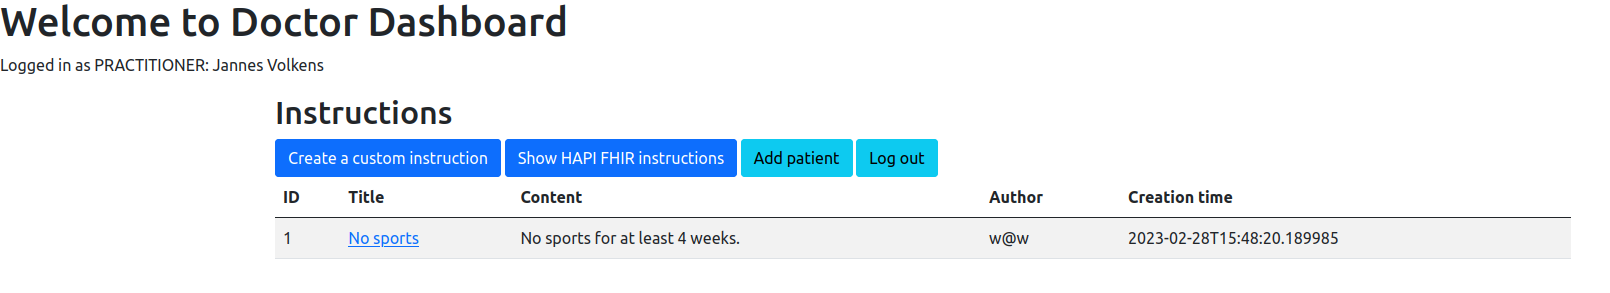
\includegraphics[width=1\textwidth]{Practitioner_Dashboard.png}
    \caption{Practitioner dashboard with one instruction present.}
    \label{fig:practitioner_dashboard}
\end{figure}
If a new patient user is to be created, a few pieces of information that are important for the creation of a new user must be specified and transmitted to the Practitioner Controller via a POST request (see Figure \ref{fig:add_patient}). The most important information is the FHIR-ID of the respective patient, which should be available to the Practitioners according to Charité. With the help of this FHIR-ID the resources for the patient as well as the Encounter and Conditions can be obtained from the FHIR server (see Listing \ref{lst:get_condition}).
\begin{lstlisting}[language=Java, label=lst:get_condition, caption={Example how to fetch the conditions for a specific FHIR ID.}]
Bundle bundle = this.client
                .search()
                .forResource(Condition.class)
                .where(Condition.ENCOUNTER.hasId(fhirID))
                .returnBundle(Bundle.class)
                .execute();
\end{lstlisting}
By the FHIR-ID one receives thus access to the entire patient data, which are important for the creation of a new patient user. It is important that when a patient is created, only the last Encounter and the associated Conditions are loaded, since this is the most current Encounter and the instructions should of course only apply to the current treatment. For this purpose, the required previously added instructions can be selected when creating a patient user, which are then assigned to the respective patients and Encounter. A Practitioner also has the option to attach a doctor's letter in the form of a PDF file to the respective Patient-User, which is then also tied to the most current Encounter and can be downloaded by the patient later. Patients will also be able to provide feedback on how they are doing after treatment. For this purpose, it is possible to select after how many days the patients should receive a reminder and the opportunity to give feedback. This can be selected from one to three weeks (0 days are added here for testing purposes). In addition, a practitioner can still add a comment if there are notes or information for the patient that are not included in the instructions or on the doctor's letter.\\
\begin{figure}[h]
    \centering
    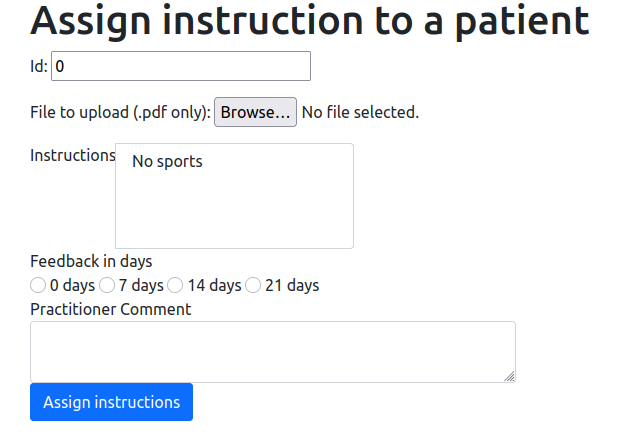
\includegraphics[width=0.6\textwidth]{Add_Patient.png}
    \caption{Interface to add a new patient.}
    \label{fig:add_patient}
\end{figure}
When the PractitionerController receives a POST request to create a patient, it first loads the patient's data from the server using the FHIR ID. In the minimal implementation this includes e.g. only the name, resourceType and the FHIR-ID, but there can be more information like birthday, address, if the Encounter is already completed, etc.. If the ID does not exist or if the patient does not have Encounter or Conditions, an error will occur and no patient will be created. Otherwise, a new user is created with the role Patient and the information from the FHIR entries. In addition, a password is generated for the patient, which consists of the name, the year of birth and a four-digit random number (example: Erika\_Mustermann\_2000\_1234). When saving the new patient in the database, a user instance is saved with the entire user-specific information and also a patient instance with the patient-specific information. In addition, the encounters with the respective conditions and instructions are stored in the database. It also creates a QR code that leads to the service's login page, which patients can scan at home for easy access. The QR code to the link is created using ZXing ("Zebra Crossing") \cite{zxing} a barcode scanning library for Java, which is then saved in a PNG file with the patient FHIR ID as name. When the patient has been created, there is once again an overview in which the FHIR ID of the patient can be seen and the respective password. If the patient user already exists and if there is a new encounter for this patient, the patient and his encounters, instructions and doctor's letter will be updated, otherwise nothing will happen.

\subsection{Patient}
As a patient, one has the ability to view their Encounter and associated Conditions and Instructions, as well as download the doctor's letter for that Encounter, which is handled by the \textit{PatientController}. In addition, patients can provide feedback to indicate how they are doing and view relevant emergency phone numbers.\\
A patient's dashboard consists of a list containing the patient's various encounters, starting with the most recent encounter (see Figure \ref{fig:patient_dashboard}). For each encounter, there is a timestamp of when it occurred, the associated conditions (diagnoses), the instructions assigned by the practitioner, the practitioner's comment (if given), when they can provide feedback on their condition, and a button to download the doctor's letter. The download of the doctor's letter is a GET request to the PatientController where the corresponding file is loaded in Blob format (Binary Large Objects), converted into a resource, and returned as a response. For the instructions, the list only shows the respective titles, but these are links to a separate view of the instructions where the content of the instruction can be found. This Encounter list is obtained by a GET request to the PatientController, which responds with the list and the content displayed there from the corresponding databases.\\
When the time comes to provide feedback for an Encounter, a note is displayed on the page for the patient to read which Encounter requires feedback. Now, in the Encounter entry, patients have the option to choose between five different ratings: from Significantly worse to Significantly better. They can also add a comment to the feedback for Charité about their condition.

\begin{figure}[h]
    \centering
    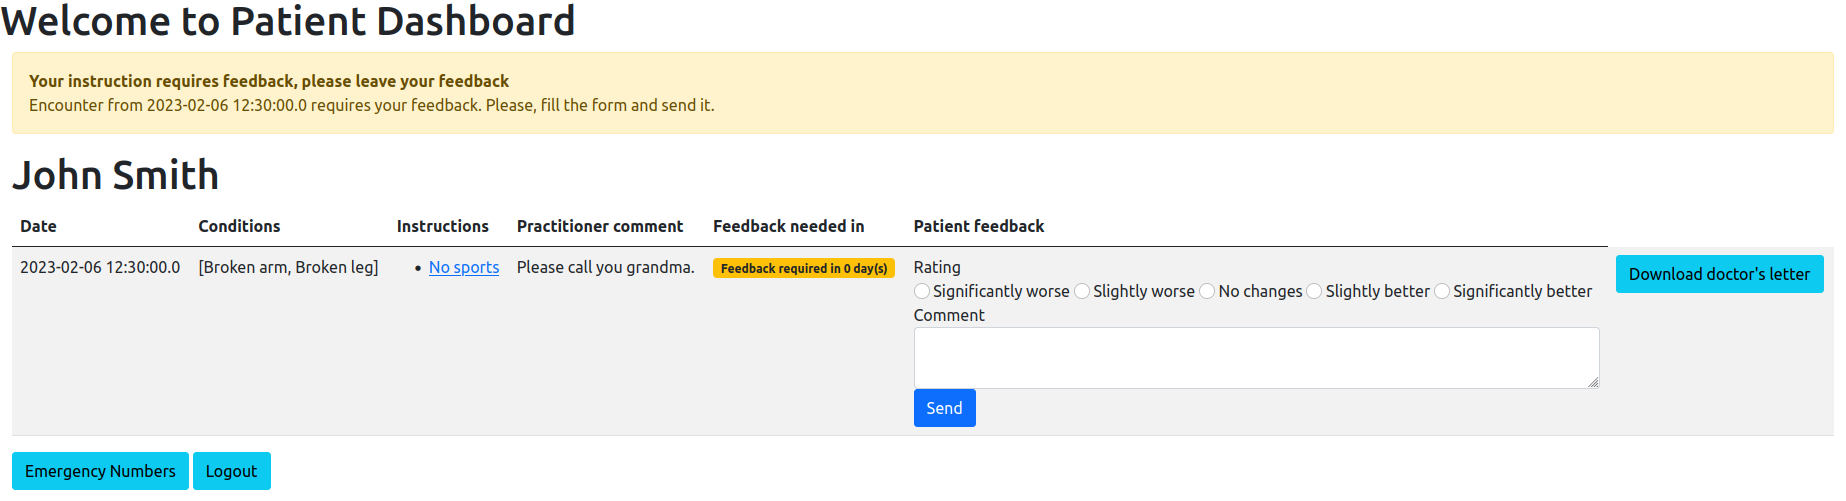
\includegraphics[width=1\textwidth]{Patient_Dashboard.png}
    \caption{Patient dashboard with one encounter present.}
    \label{fig:patient_dashboard}
\end{figure}

\subsection{Frontend}
Note: The screenshots in this report show a frontend, which was implemented purely for testing purposes and does not contribute to the functionality of the backend, which is why it is not discussed in detail.

\section{Conclusion}
This project shows that it is possible to create a system that allows potential patients to receive their instructions and doctor's letters in digital form. The system is able to manage different users with different roles, who have their own views with user-specific data and can share data with each other. As an admin, all users can manage, whereas practitioners can create new patients and assign instructions as well as doctor's letters to them. Patients can view this data and send feedback to the admins.\\
\textbf{Outlook}\\
To expand the system even further, it would be possible to establish a connection to the front end of another project group. In addition, the feedback function can be expanded to include other items, such as feedback on hospitalization and use of the app. Moreover, a reminder function would be useful, with the help of which patients could be reminded of subsequent doctor visits. Finally, it would be conceivable to publish the server and connect it to the hospital system of the Charité, since the service currently only runs locally, although questions would then arise regarding data privacy.

\section{Reflection}

\bibliography{literature.bib}{}
\bibliographystyle{plain}
\end{document}
